\documentclass[a4paper]{article}
\usepackage[utf8]{inputenc}
\usepackage{graphicx} % Required for including images
\usepackage[font=small,labelfont=bf]{caption}
\usepackage{courier}
\usepackage{amsmath}
\usepackage{color}
\usepackage{listings}
\usepackage{subcaption}
\usepackage[table,xcdraw]{xcolor}

\usepackage{array}
\newcolumntype{M}[1]{>{\centering\arraybackslash}m{#1}}

\lstset{
    basicstyle=\ttfamily,
    language=Octave,
    morecomment = [l][\itshape\color{blue}]{\%}
}

\addtolength{\oddsidemargin}{-.875in}
\addtolength{\evensidemargin}{-.875in}
\addtolength{\textwidth}{1.75in}

\addtolength{\topmargin}{-.875in}
\addtolength{\textheight}{1.75in}

\setlength{\parindent}{0pt}
\setlength{\parskip}{0.5em}

\renewcommand{\figurename}{Figura}
\renewcommand{\tablename}{Tabla}

\newcommand{\bold}[1]{\textbf{\texttt{#1}}}

\title{TP 2: Algoritmos de Clasificación Supervisada}
\author{Giuliano Scaglioni}
\date{Septiembre 2019}

\begin{document}

\clearpage\maketitle
\thispagestyle{empty}

\newpage

\setcounter{page}{1}

\section{Deportes en el río}
  \subsection{Implementación}
  La implementación del programa se realizó en Go utilizando el algoritmo ID3 para construir el árbol de decision.

  \subsubsection{Entidades}
    En la implementación se definieron las siguientes entidades
    \begin{itemize}
      \item \bold{Classifier}: es una abstracción de un clasificador. Define una interfaz que permite clasificar un ejemplo. Cada clasificador implementado en el trabajo práctico, implementa esta interfaz.
      \item \bold{Metric}: es un tipo que almacena metricas de evaluación de un clasificador. Además provee metodos para evaluar un clasificador independientemente de su implementación.
      \item \bold{Example}: representa un ejemplo, su implementación es un mapa donde cada entrada tiene como clave el nombre del atributo y como valor, el valor que tiene ese atributo en el ejemplo.
      \item \bold{DecisionTree}: representa un árbol de decisión, para crear uno, se pasa una lista de ejemplos y el nombre del atributo a predecir. La implementación interna de esta entidad utiliza el algoritmo ID3 para crearlo. En la creación de un árbol de decisión, a su vez, se utilizan otras entidades, estas son:
      \begin{itemize}
        \item \bold{Node}: representa un nodo del arbol de decisión y define comportamiento para obtener el tipo de nodo, obtener la lista de hijos de este, agregar hijos, entre otros métodos necesarios para su representación.
        \item \bold{AttrNode}: es una implementación de Node para los nodos que representan un atributo.
        \item \bold{ValNode}: es una implementación de Node para los nodos que representan los valores posibles de un atributo.
        \item \bold{ClassNode}: es una implementación de Node para los nodos que representan una clase. Esta implementación no permite agregar hijos pues este tipo de nodos siempre es hoja.
      \end{itemize}
    \end{itemize}
  \subsubsection{Visualización del árbol}
    El programa implementado construye el árbol a partir de una lista de examples y el atributo a predecir, y genera como salida el árbol en formato Graphviz dot. 

    Además se provee una utilidad implementada en Vue.js que permite crear el árbol a partir de un archivo csv y visualizar el árbol de decisión desde el navegador utilizando como backend el programa implementado.
\subsection{Árboles de decisión}
Se utilizó el programa descripto anteriormente para construír el árbol de decisión para el conjunto de datos provisto.

\begin{figure}[h]
  \centering
    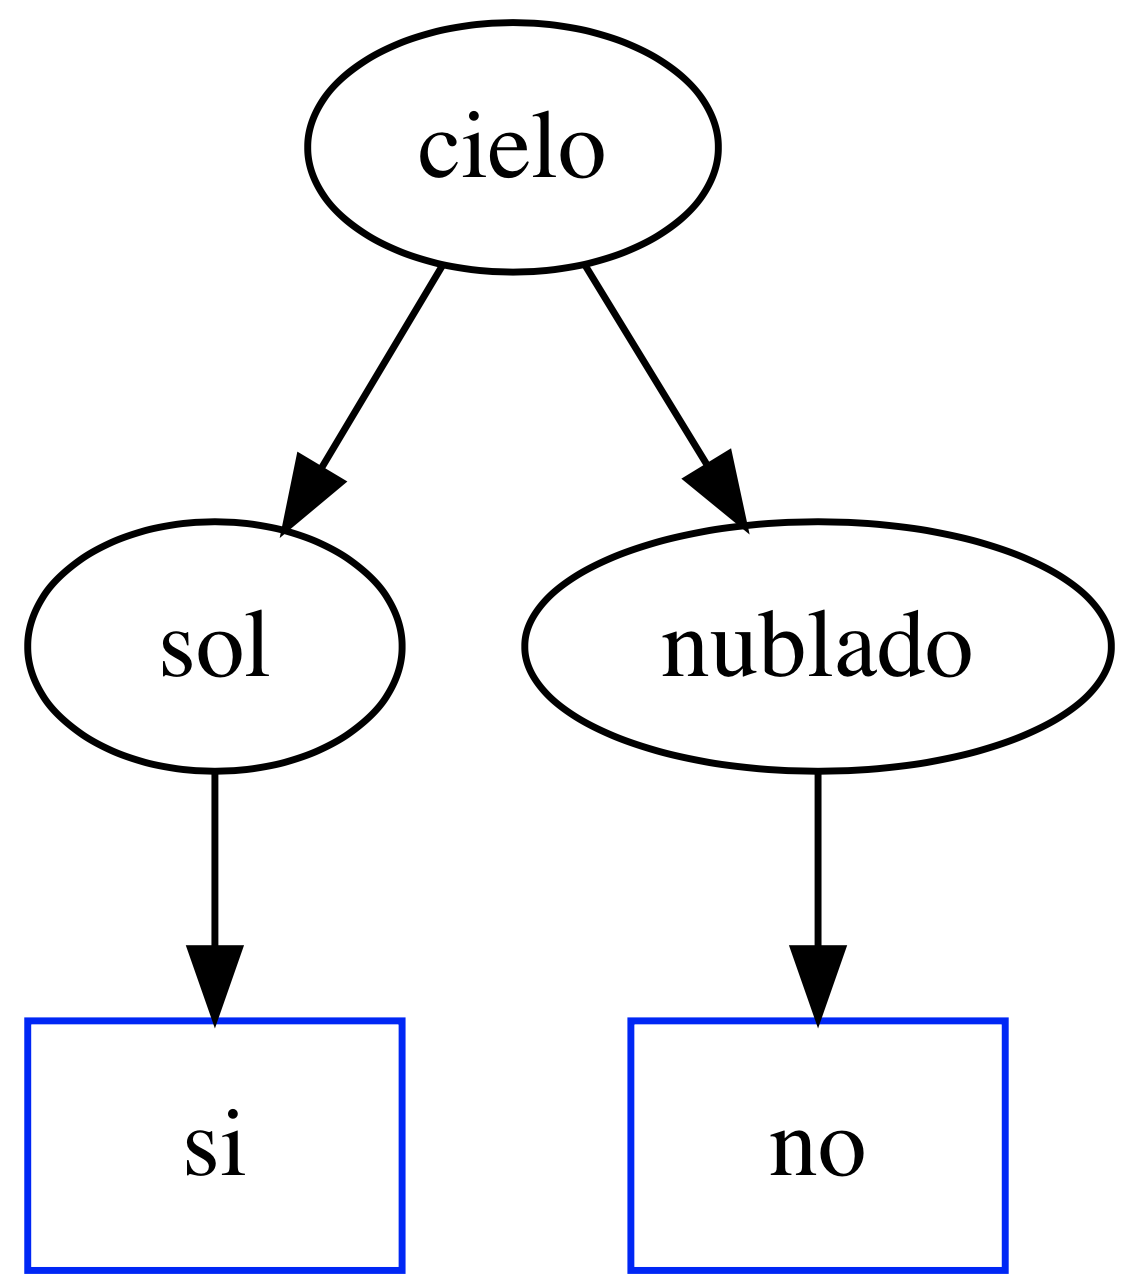
\includegraphics[scale=0.2]{img/tree1.png}
  \caption{Árbol de decisión construído.}
  \label{ej1-tree1}
\end{figure}

Como se puede observar en la Fig. \ref{ej1-tree1}, los únicos atributos relevantes para determinar si la persona disfruta de deportes en el río son el cielo y la temperatura. En la implementación del algoritmo \bold{ID3} se decidió que, en casos de empte, se conserve el primer atributo evaluado, en este caso, cielo.

Si se compara con los datos de la Tabla \ref{tab:dataset-1}, se puede ver que coincide en que, para determinar si disfruta, el atributo cielo tiene que tener el valor sol.

\begin{table}[h]
  \centering
  \begin{tabular}{ccccccc}
  Cielo                          & Tempe. & Humedad & Viento & Agua   & Pronós.    & ¿Disfruta?                \\ \hline
  {\color[HTML]{009901} sol}     & calida & normal  & fuerte & calida & estable   & {\color[HTML]{009901} si} \\
  {\color[HTML]{009901} sol}     & calida & alta    & fuerte & calida & estable   & {\color[HTML]{009901} si} \\
  {\color[HTML]{CB0000} nublado} & frio   & alta    & fuerte & calida & cambiante & {\color[HTML]{CB0000} no} \\
  {\color[HTML]{009901} sol}     & cálida & alta    & fuerte & fria   & cambiante & {\color[HTML]{009901} si}
  \end{tabular}
  \caption{Conjunto de datos provisto}
  \label{tab:dataset-1}
  \end{table}

Al agregar el nuevo ejemplo indicado se obtuvo el árbol de decisión de la Figura \ref{ej1-tree2}.

\begin{figure}[h]
  \centering
    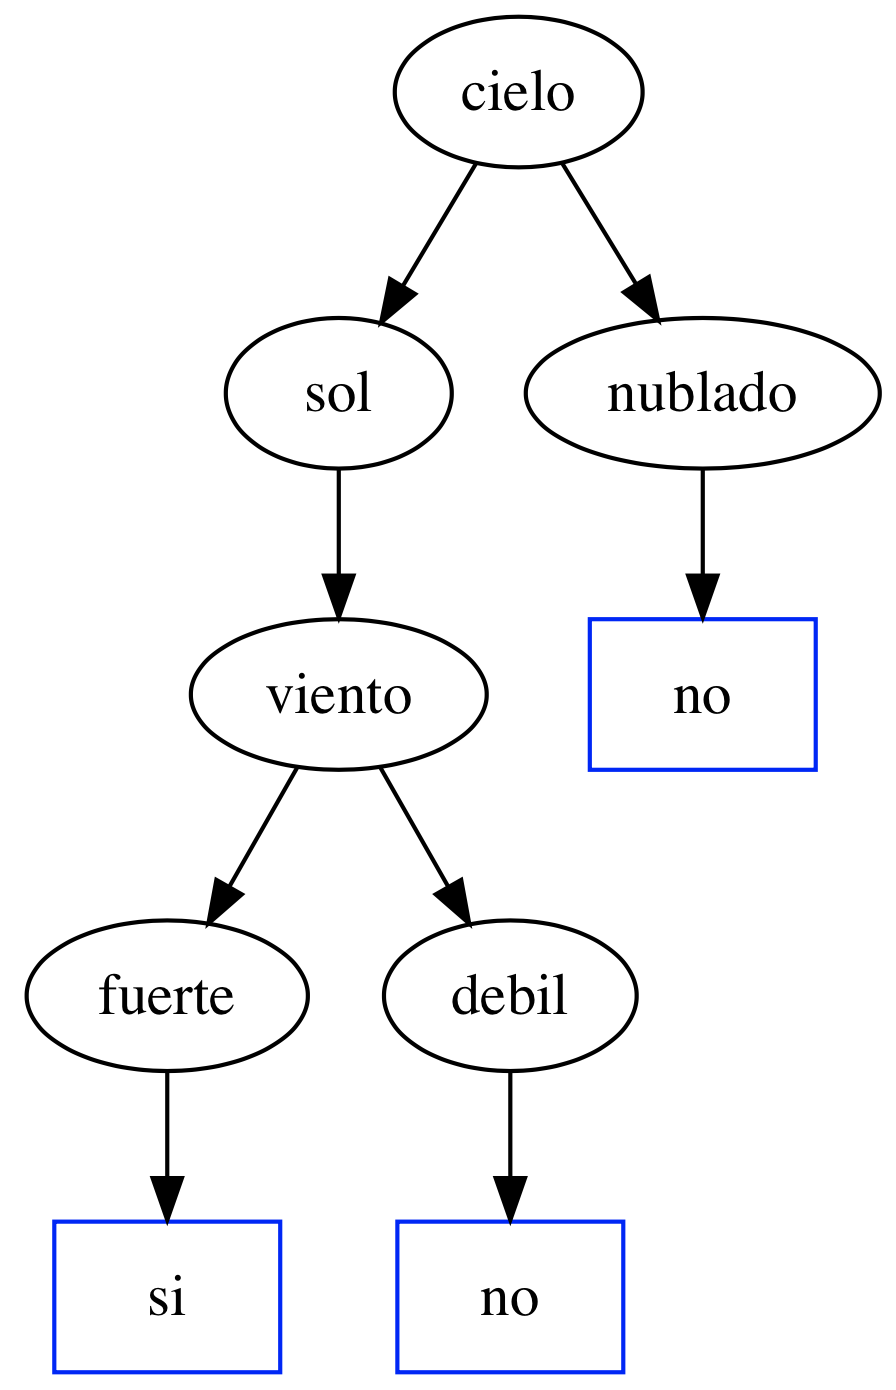
\includegraphics[scale=0.4]{img/tree2.png}
  \caption{Árbol de decisión construído.}
  \label{ej1-tree2}
\end{figure}

Como se puede observar en la Tabla \ref{tab:dataset-2}, en caso de que el atributo cielo sea sol tambien se debe comprobar el valor del atributo viento para determinar si disfruta, lo cual coincide con el árbol de decisión obtenido.

\begin{table}[h]
  \centering
  \begin{tabular}{ccccccc}
  Cielo                          & Tempe. & Humedad & Viento                        & Agua   & Pronós.    & ¿Disfruta?                \\ \hline
  {\color[HTML]{009901} sol}     & calida & normal  & {\color[HTML]{009901} fuerte} & calida & estable   & {\color[HTML]{009901} si} \\
  {\color[HTML]{009901} sol}     & calida & alta    & fuerte                        & calida & estable   & {\color[HTML]{009901} si} \\
  {\color[HTML]{CB0000} nublado} & frio   & alta    & fuerte                        & calida & cambiante & {\color[HTML]{CB0000} no} \\
  {\color[HTML]{009901} sol}     & calida & alta    & fuerte                        & fria   & cambiante & {\color[HTML]{009901} si} \\
  {\color[HTML]{009901} sol}     & calida & normal  & {\color[HTML]{CB0000} debil}  & calida & estable   & {\color[HTML]{CB0000} no}
  \end{tabular}
  \caption{Conjunto de datos con el ejemplo agregado}
  \label{tab:dataset-2}
  \end{table}
    
\end{document}
